\chapter{Conclusion}
This thesis tested and analyzed a Fully Convolutional Network (FCN) for segmenting facial images under occlusion. This standard network was trained by Nirkin et al. \cite{nirkin2018_faceswap} on a rich and diverse dataset. They claim that the speed and the accuracy of this segmentation method outperforms other approaches that were made especially for this task.\\
\\
We evaluate the segmentation accuracy of the network on two real-life datasets. In one of them, every image was supplied with the ground truth labels, which determine whether a pixel belongs to the face or not. A comparison of both segmentations showed that the segmentation of the FCN contained very few false positives. However, the FCN only recognizes about 4/5 of the actual facial region (false negatives). In a further step, we evaluated the network on synthetic images with a to be able to be in control of all parameters ourselves. The results show that there is a hierarchy among the angles that determine the position of the face. There is a hierarchy among the angles that determine the position of the face. Regardless of whether the face is hidden or not, the FCN the most vulnerable to large roll-angles, then pitch-angles and least important are the yaw-angles. That's a strange result, because no matter how the face is rolled, the information does not change. We fear that the reason for this is the training of the FCN. 

\begin{figure}
	\centering
	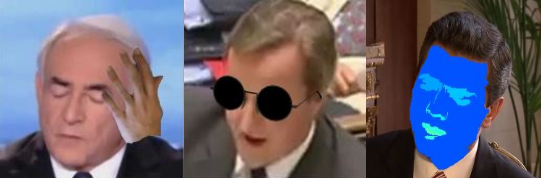
\includegraphics[width=0.5\textwidth]{Figures/chap5/tran_frames.png}
	\caption{Three examples of training images used by Nirkin et al. These are pictures of the recent Janus CS2 dataset. It looks like the face was not turned on any of the faces. The first two images are overlayd with synthetic occlusions. The third one depicts the interface used for semi-supervised labeling.}
	\label{fig:chap5:train_images}
\end{figure}

Egger et al. \cite{egger_paper} of the University of Basel propose an EM-like method to simultaneously segment a face out of a given image and reconstruct it. We compare the segmentations of Egger et al. with the segmentation of the FCN and find that (1) The approach of Egger et al. oversegments the image, (2) The method of Egger et al. tends to exclude important details like the eyes due to they strong variability in color and shape, (3) The FCN often fails in recognizing and segmenting thin occlusions.\\
\\
The runtime of the FCN is much faster compared with the iterative segmentation of Egger et al. On our GPU, the segmentation with the FCN takes approximately 3 seconds, while the algorithm of Egger et al. takes 2 minutes (according to \cite{egger_paper}).

\begin{figure}
\centering
\subbottom[original]{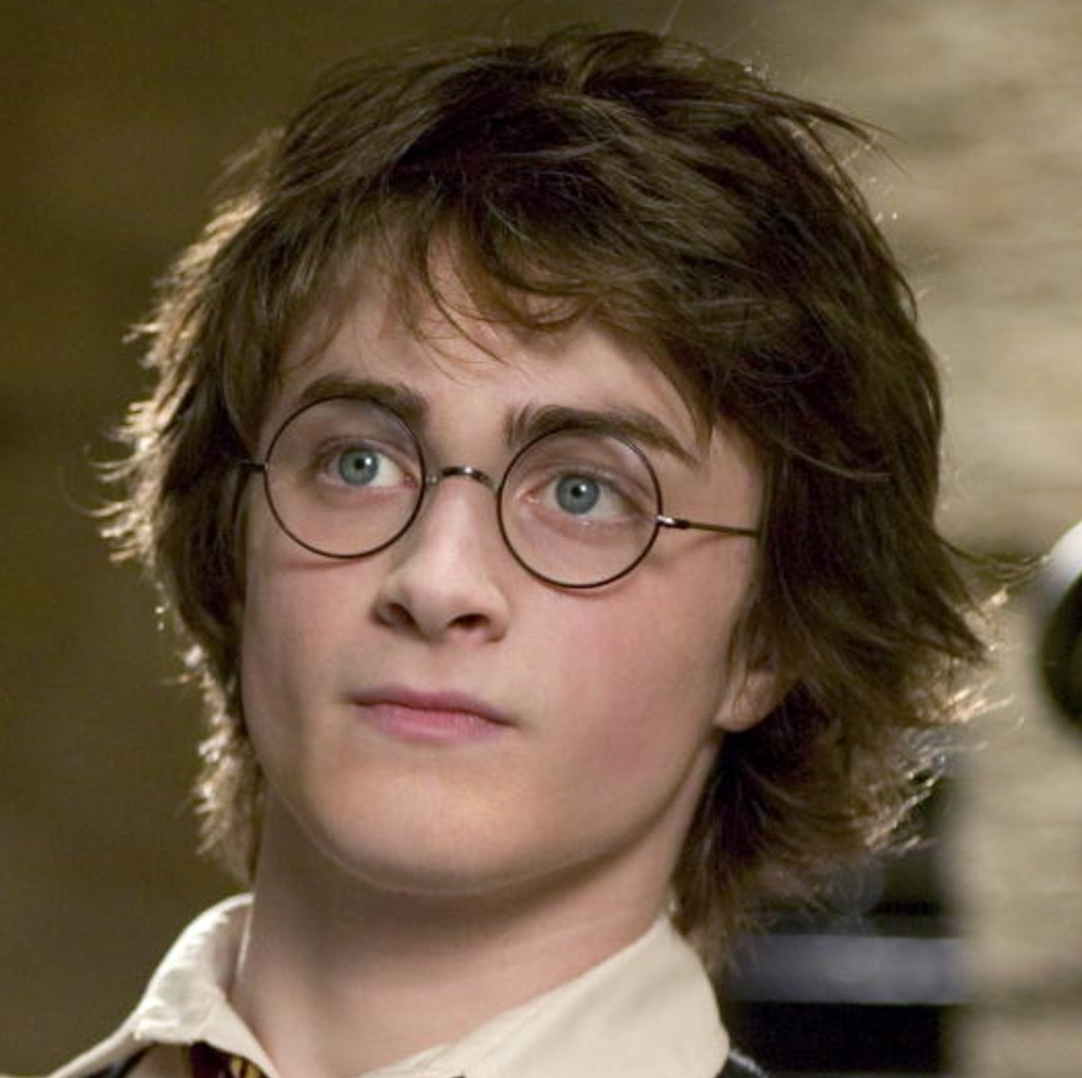
\includegraphics[width=0.2\textwidth]{Figures/chap5/harry_original.png}\label{fig:tm:tm1}}
\subbottom[segmentation of Egger et al.]{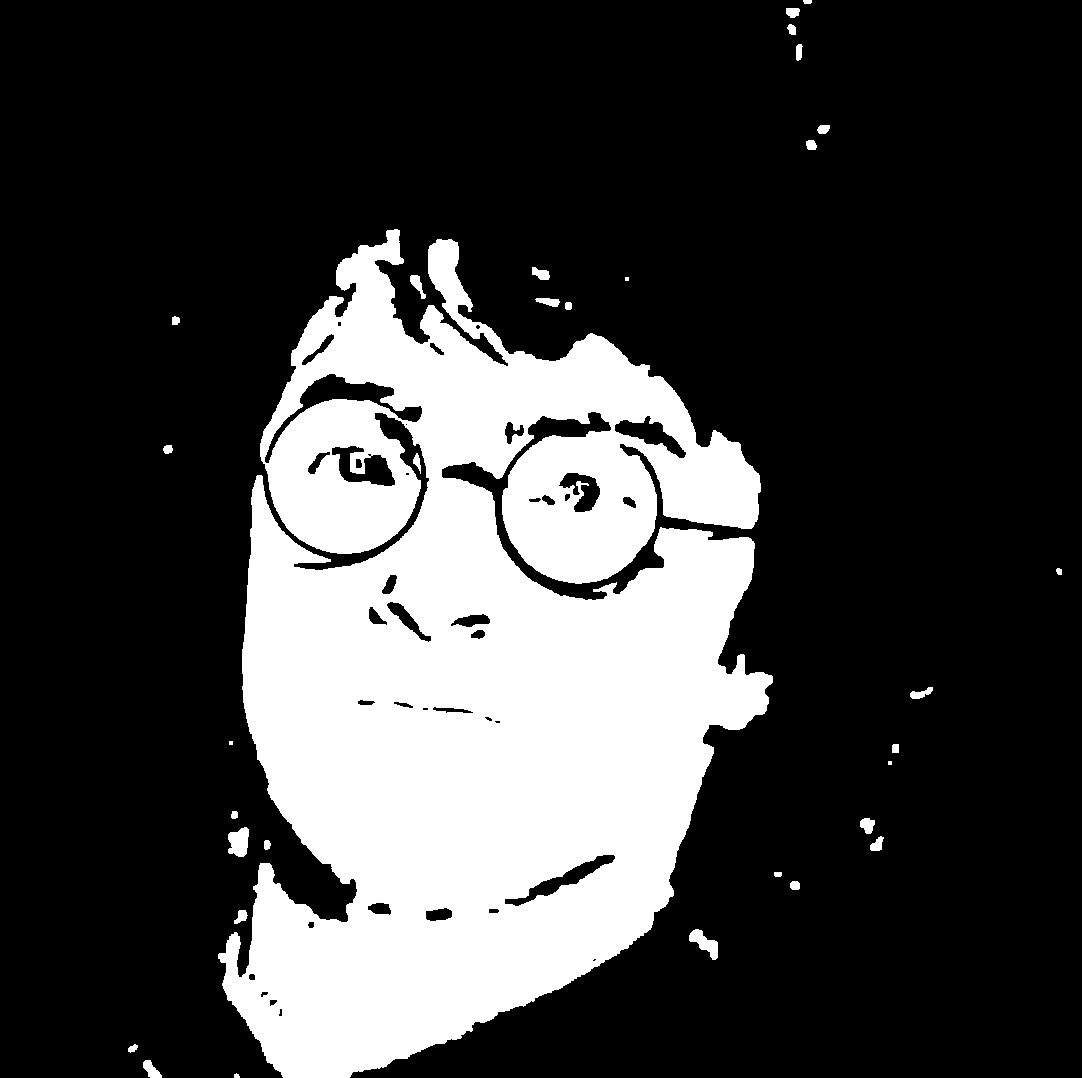
\includegraphics[width=0.2\textwidth]{Figures/chap4/harry_mask_EGGER_.png}\label{fig:tm:tm2}}
\subbottom[segmentation of FCN]{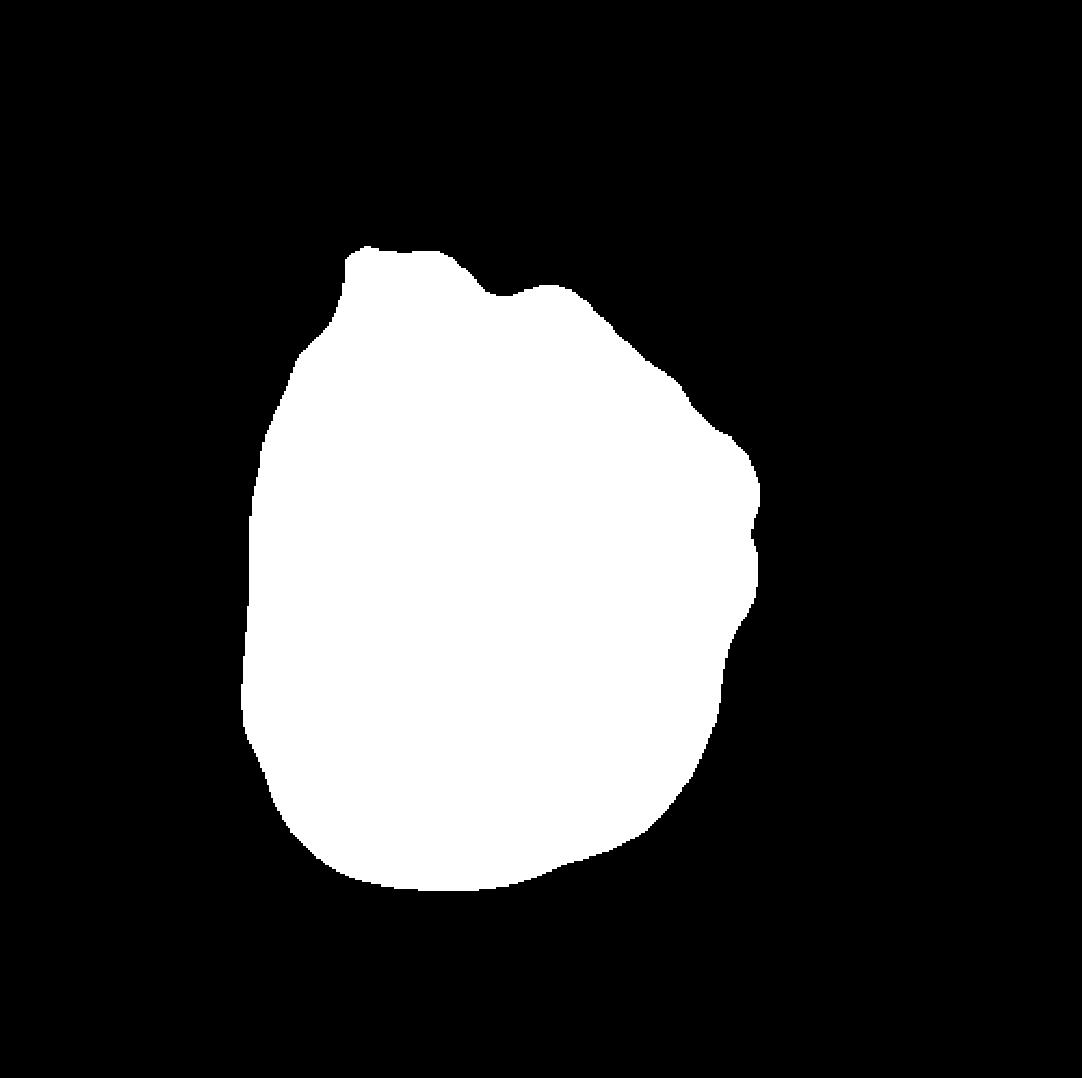
\includegraphics[width=0.2\textwidth]{Figures/chap4/harry_mask_FCN_.png}\label{fig:tm:tm3}}
\caption{Comparison of the two segmentation ((b) and (c)) of the same facial image (a).}
\label{fig:chap5:harry}
\end{figure}

Both approaches have their weaknesses and strengths, which we try to combine. Therefore we take the iterative algorithm of Egger et al. and give it the FCN-Segmentation as an initial segmentation. Since this algorithm uses a Metropolis-Hastings method, the final mask looks very similar to Egger et al.'s mask without the integration. However, the illumination estimation is improved a lot, because an initial mask exists (the original approach of egger et al. does not use a mask/segmentation to determine the illumination parameters). This is an interesting starting point for further research on how to optimally combine both segmentations.